% Benchmark appendix with extended narrative and figures.
\chapter{Curriculum vs Single Benchmark v1}
\label{app:curr-vs-single-v1}

\section{Objective and motivation}

The core research question in this phase was:
\emph{Does curriculum training improve final quality, convergence behavior,
or efficiency relative to direct single-target training?}

This benchmark was designed as a controlled comparison where:

\begin{itemize}
    \item data generation settings were matched per function,
    \item hyperparameters were inherited from prior sweep best trials,
    \item only the training strategy changed (\texttt{single} vs \texttt{curriculum}).
\end{itemize}

The rationale was to evaluate whether curriculum contributes measurable value
beyond already-strong per-function hyperparameters.

\section{Experimental protocol}

\textbf{Benchmark id:} \texttt{curr\_vs\_single\_20260315\_175826}.\\
\textbf{Run window:} 2026-03-15T17:58:26+01:00 to 2026-03-16T01:10:36+01:00.\\
\textbf{Completed runs:} 96/96 (runner), 96/96 (MLflow FINISHED).

\paragraph{Factorial design.}

\begin{itemize}
    \item Methods: \texttt{single} vs \texttt{curriculum}
    \item Regimes: \texttt{equal\_epochs}, \texttt{equal\_time}
    \item Functions: 8 benchmark functions
    \item Seeds: 42, 43, 44
\end{itemize}

Total runs: \(2 \times 2 \times 8 \times 3 = 96\).

\paragraph{Primary metrics.}

\begin{itemize}
    \item final quality: \texttt{final\_hard\_val\_loss}
    \item efficiency: median runtime (seconds)
    \item secondary efficiency: time-to-target hit rate
\end{itemize}

In the delta tables, positive
\texttt{delta\_quality\_single\_minus\_curriculum} means curriculum has lower
(loss-better) median quality.

\section{Headline benchmark outcomes}

\begin{table}[h]
\centering
\small
\begin{tabular}{lrrrr}
\toprule
Regime & Quality (Curr.) & Quality (Single) & Runtime (Single) & Runtime (Curr.) \\
\midrule
equal\_epochs & 5 & 3 & 8 & 0 \\
equal\_time & 3 & 5 & 8 & 0 \\
\bottomrule
\end{tabular}
\caption{Win counts by regime.}
\label{tab:curr-vs-single-win-counts}
\end{table}

\begin{table}[h]
\centering
\small
\begin{tabular}{llll}
\toprule
Function & equal\_epochs & equal\_time & Runtime winner \\
\midrule
ackley & single & single & single \\
bukin & curriculum & curriculum & single \\
eggholder & single & single & single \\
franke & curriculum & curriculum & single \\
friedman1\_2d & curriculum & single & single \\
friedman2\_2d & curriculum & single & single \\
levy & curriculum & curriculum & single \\
peaks & single & single & single \\
\bottomrule
\end{tabular}
\caption{Quality winners by function and regime.}
\label{tab:curr-vs-single-function-winners}
\end{table}

\section{Visual diagnostics}

\begin{figure}[h]
    \centering
    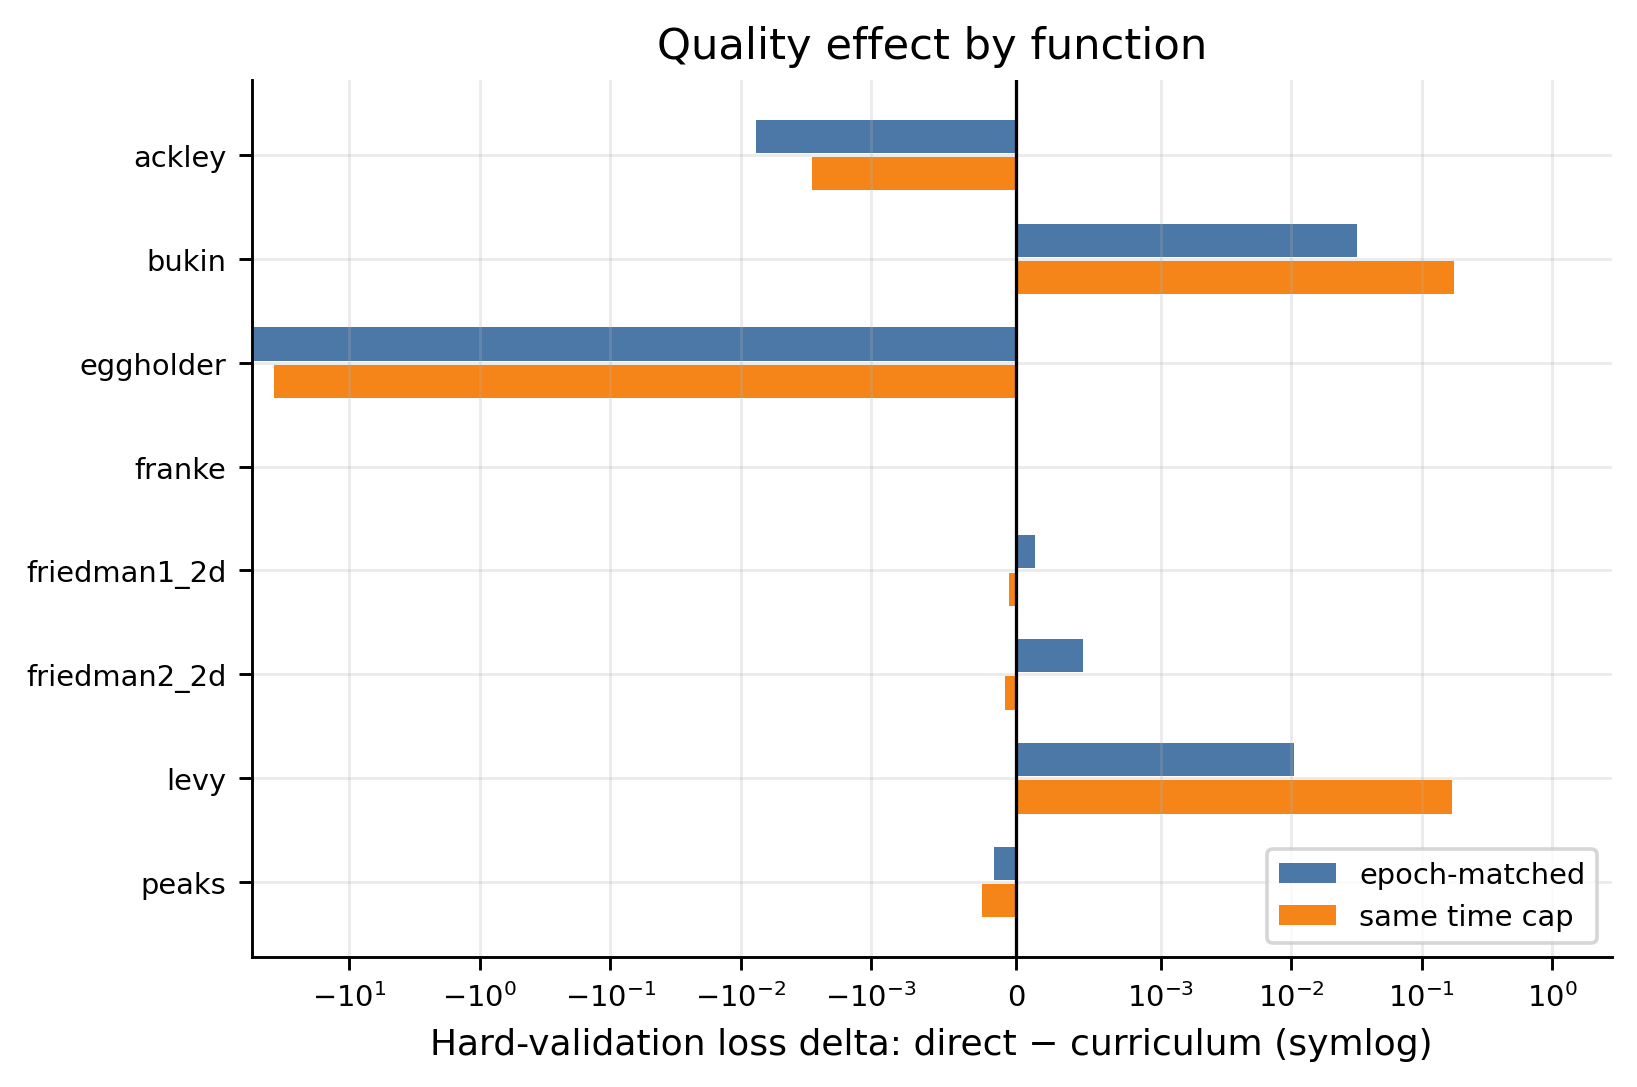
\includegraphics[width=0.95\textwidth]{figures/curr_vs_single_quality_delta.png}
    \caption{Quality delta per function (single minus curriculum). Positive bars favor curriculum.}
    \label{fig:curr-vs-single-quality-delta}
\end{figure}

\begin{figure}[h]
    \centering
    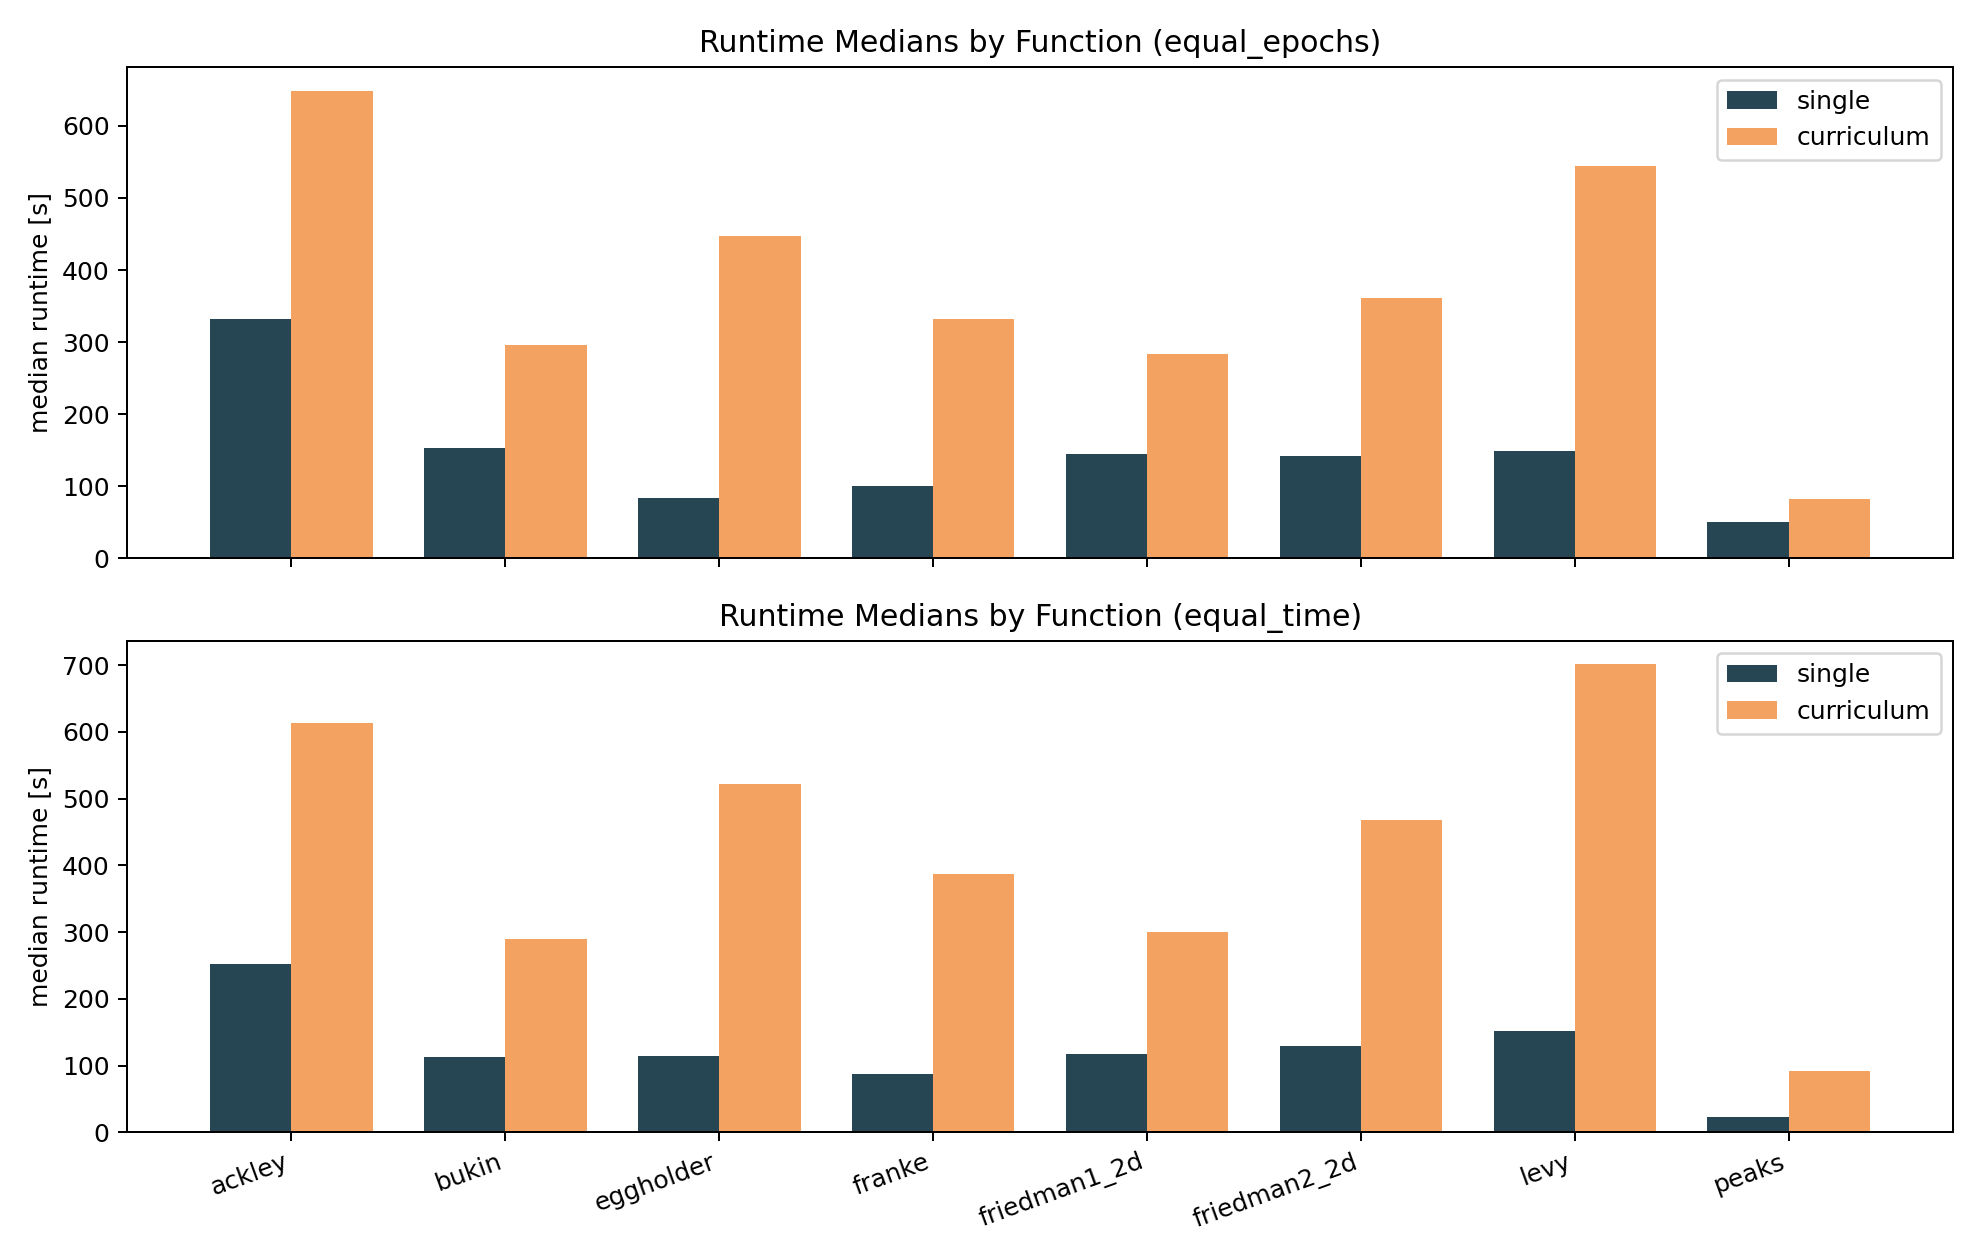
\includegraphics[width=0.95\textwidth]{figures/curr_vs_single_runtime_median.png}
    \caption{Median runtime by function and method for each regime.}
    \label{fig:curr-vs-single-runtime}
\end{figure}

\begin{figure}[h]
    \centering
    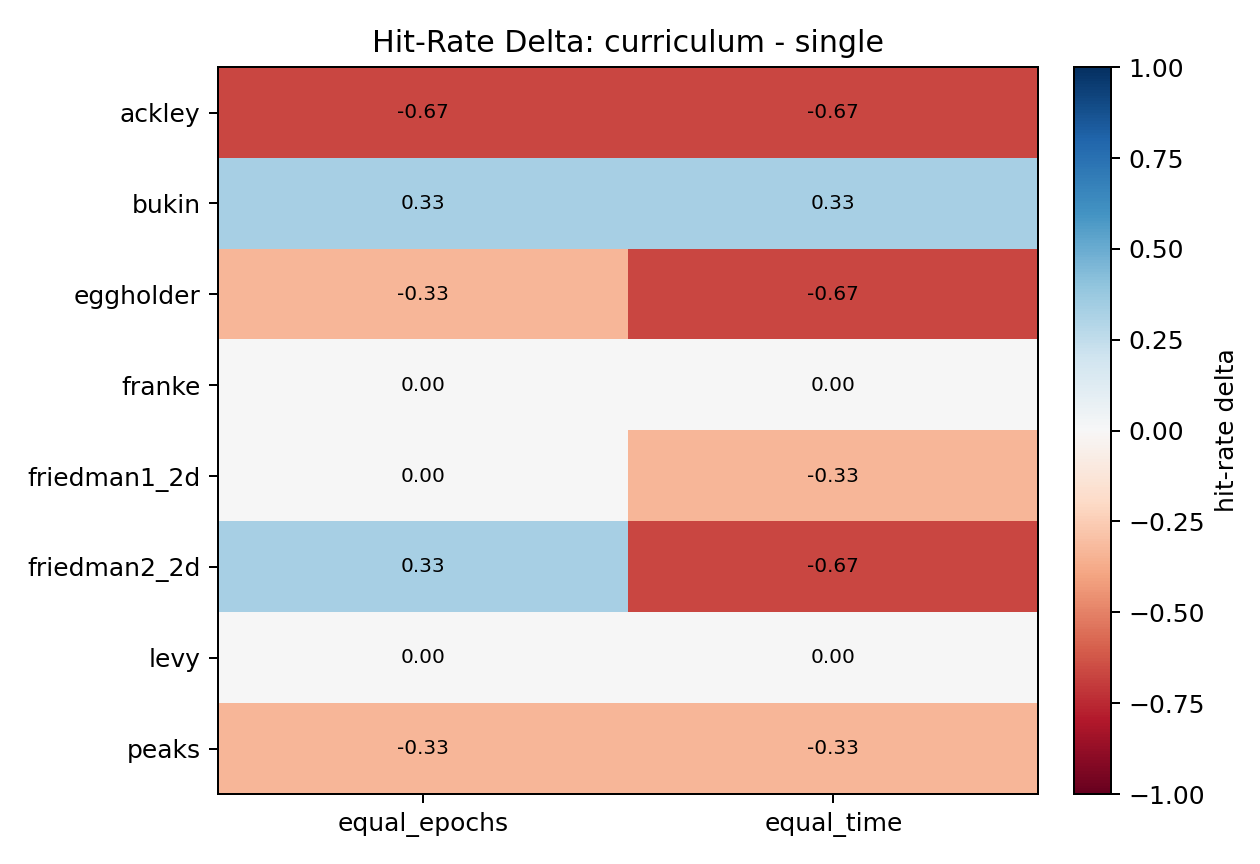
\includegraphics[width=0.72\textwidth]{figures/curr_vs_single_hitrate_delta.png}
    \caption{Time-to-target hit-rate delta (curriculum minus single). Negative values favor single.}
    \label{fig:curr-vs-single-hit-rate}
\end{figure}

\section{MLflow artifact inspection (learning dynamics)}

To inspect whether curriculum was practically useful beyond scalar summary
metrics, I additionally reviewed raw MLflow artifact plots from representative
runs (seed 42, equal\_epochs):

\begin{itemize}
    \item functions where curriculum helped quality: \texttt{bukin}, \texttt{levy},
    \item functions where curriculum did not help: \texttt{ackley}, \texttt{eggholder}.
\end{itemize}

The following figures are assembled directly from MLflow artifacts logged during
training (parent-run global metrics, child-run snapshots, and parent-run stage
surfaces).

\begin{figure}[h]
    \centering
    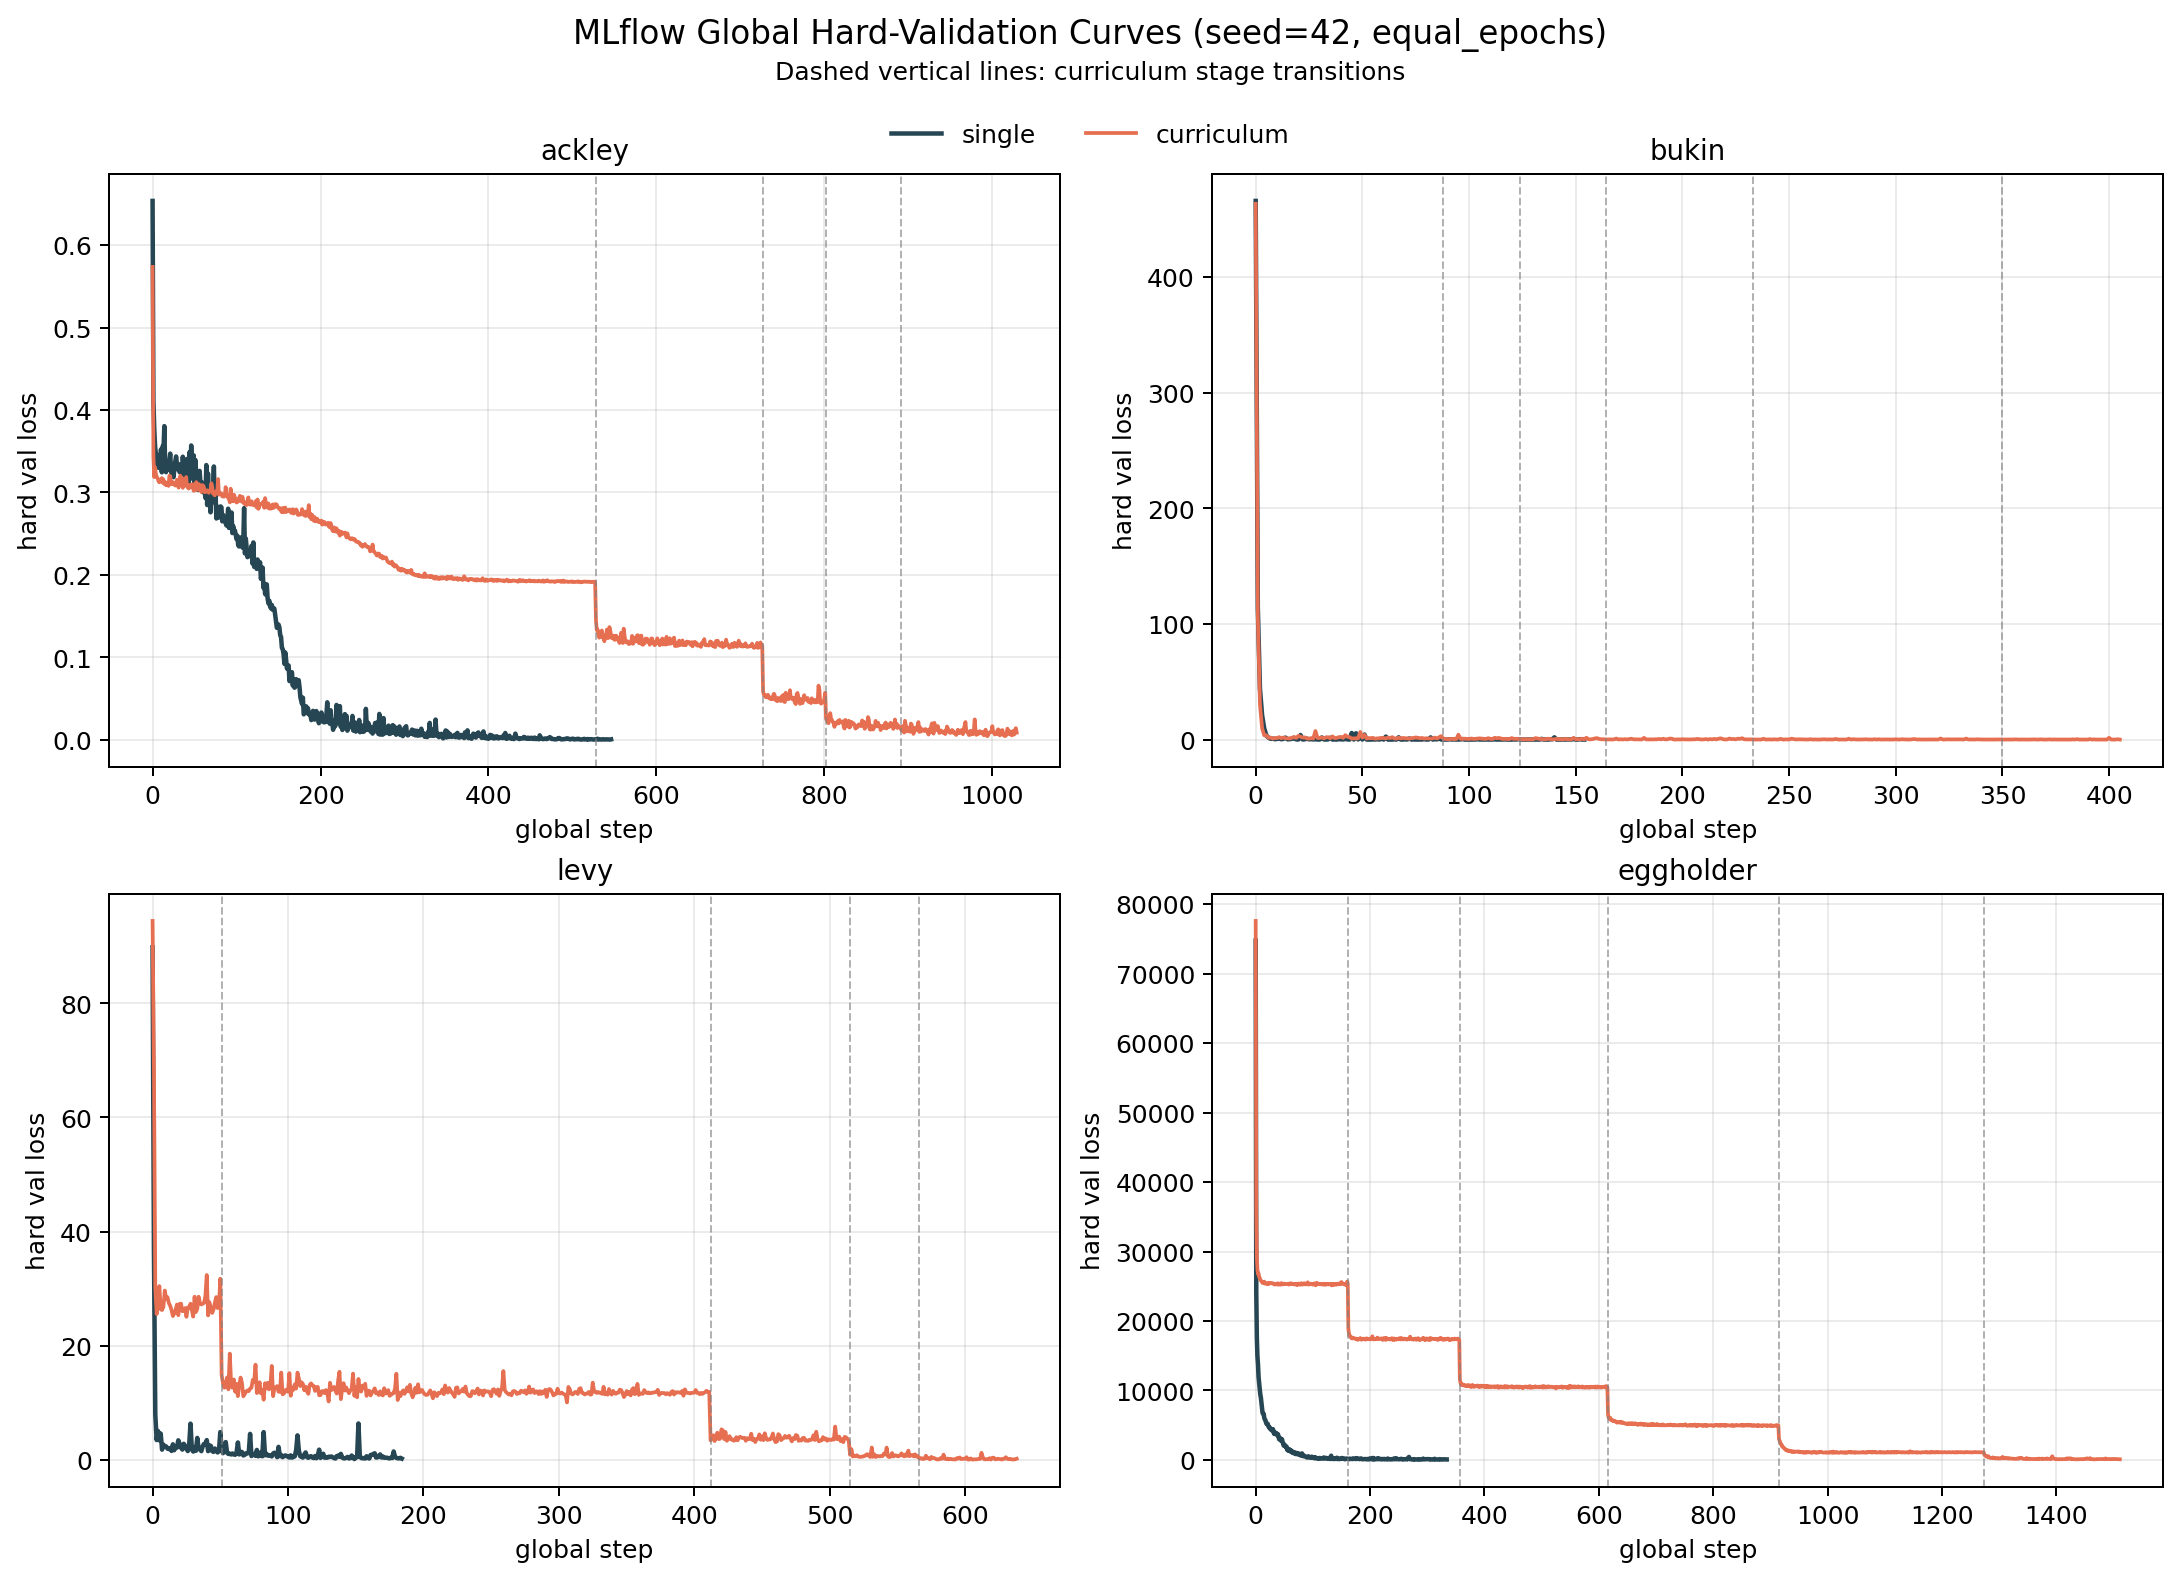
\includegraphics[width=0.98\textwidth]{figures/mlflow_curr_vs_single_global_hardval_seed42.png}
    \caption{MLflow parent-run global hard-validation curves (single vs curriculum). Dashed vertical lines mark curriculum stage transitions.}
    \label{fig:mlflow-learning-curves}
\end{figure}

\begin{figure}[h]
    \centering
    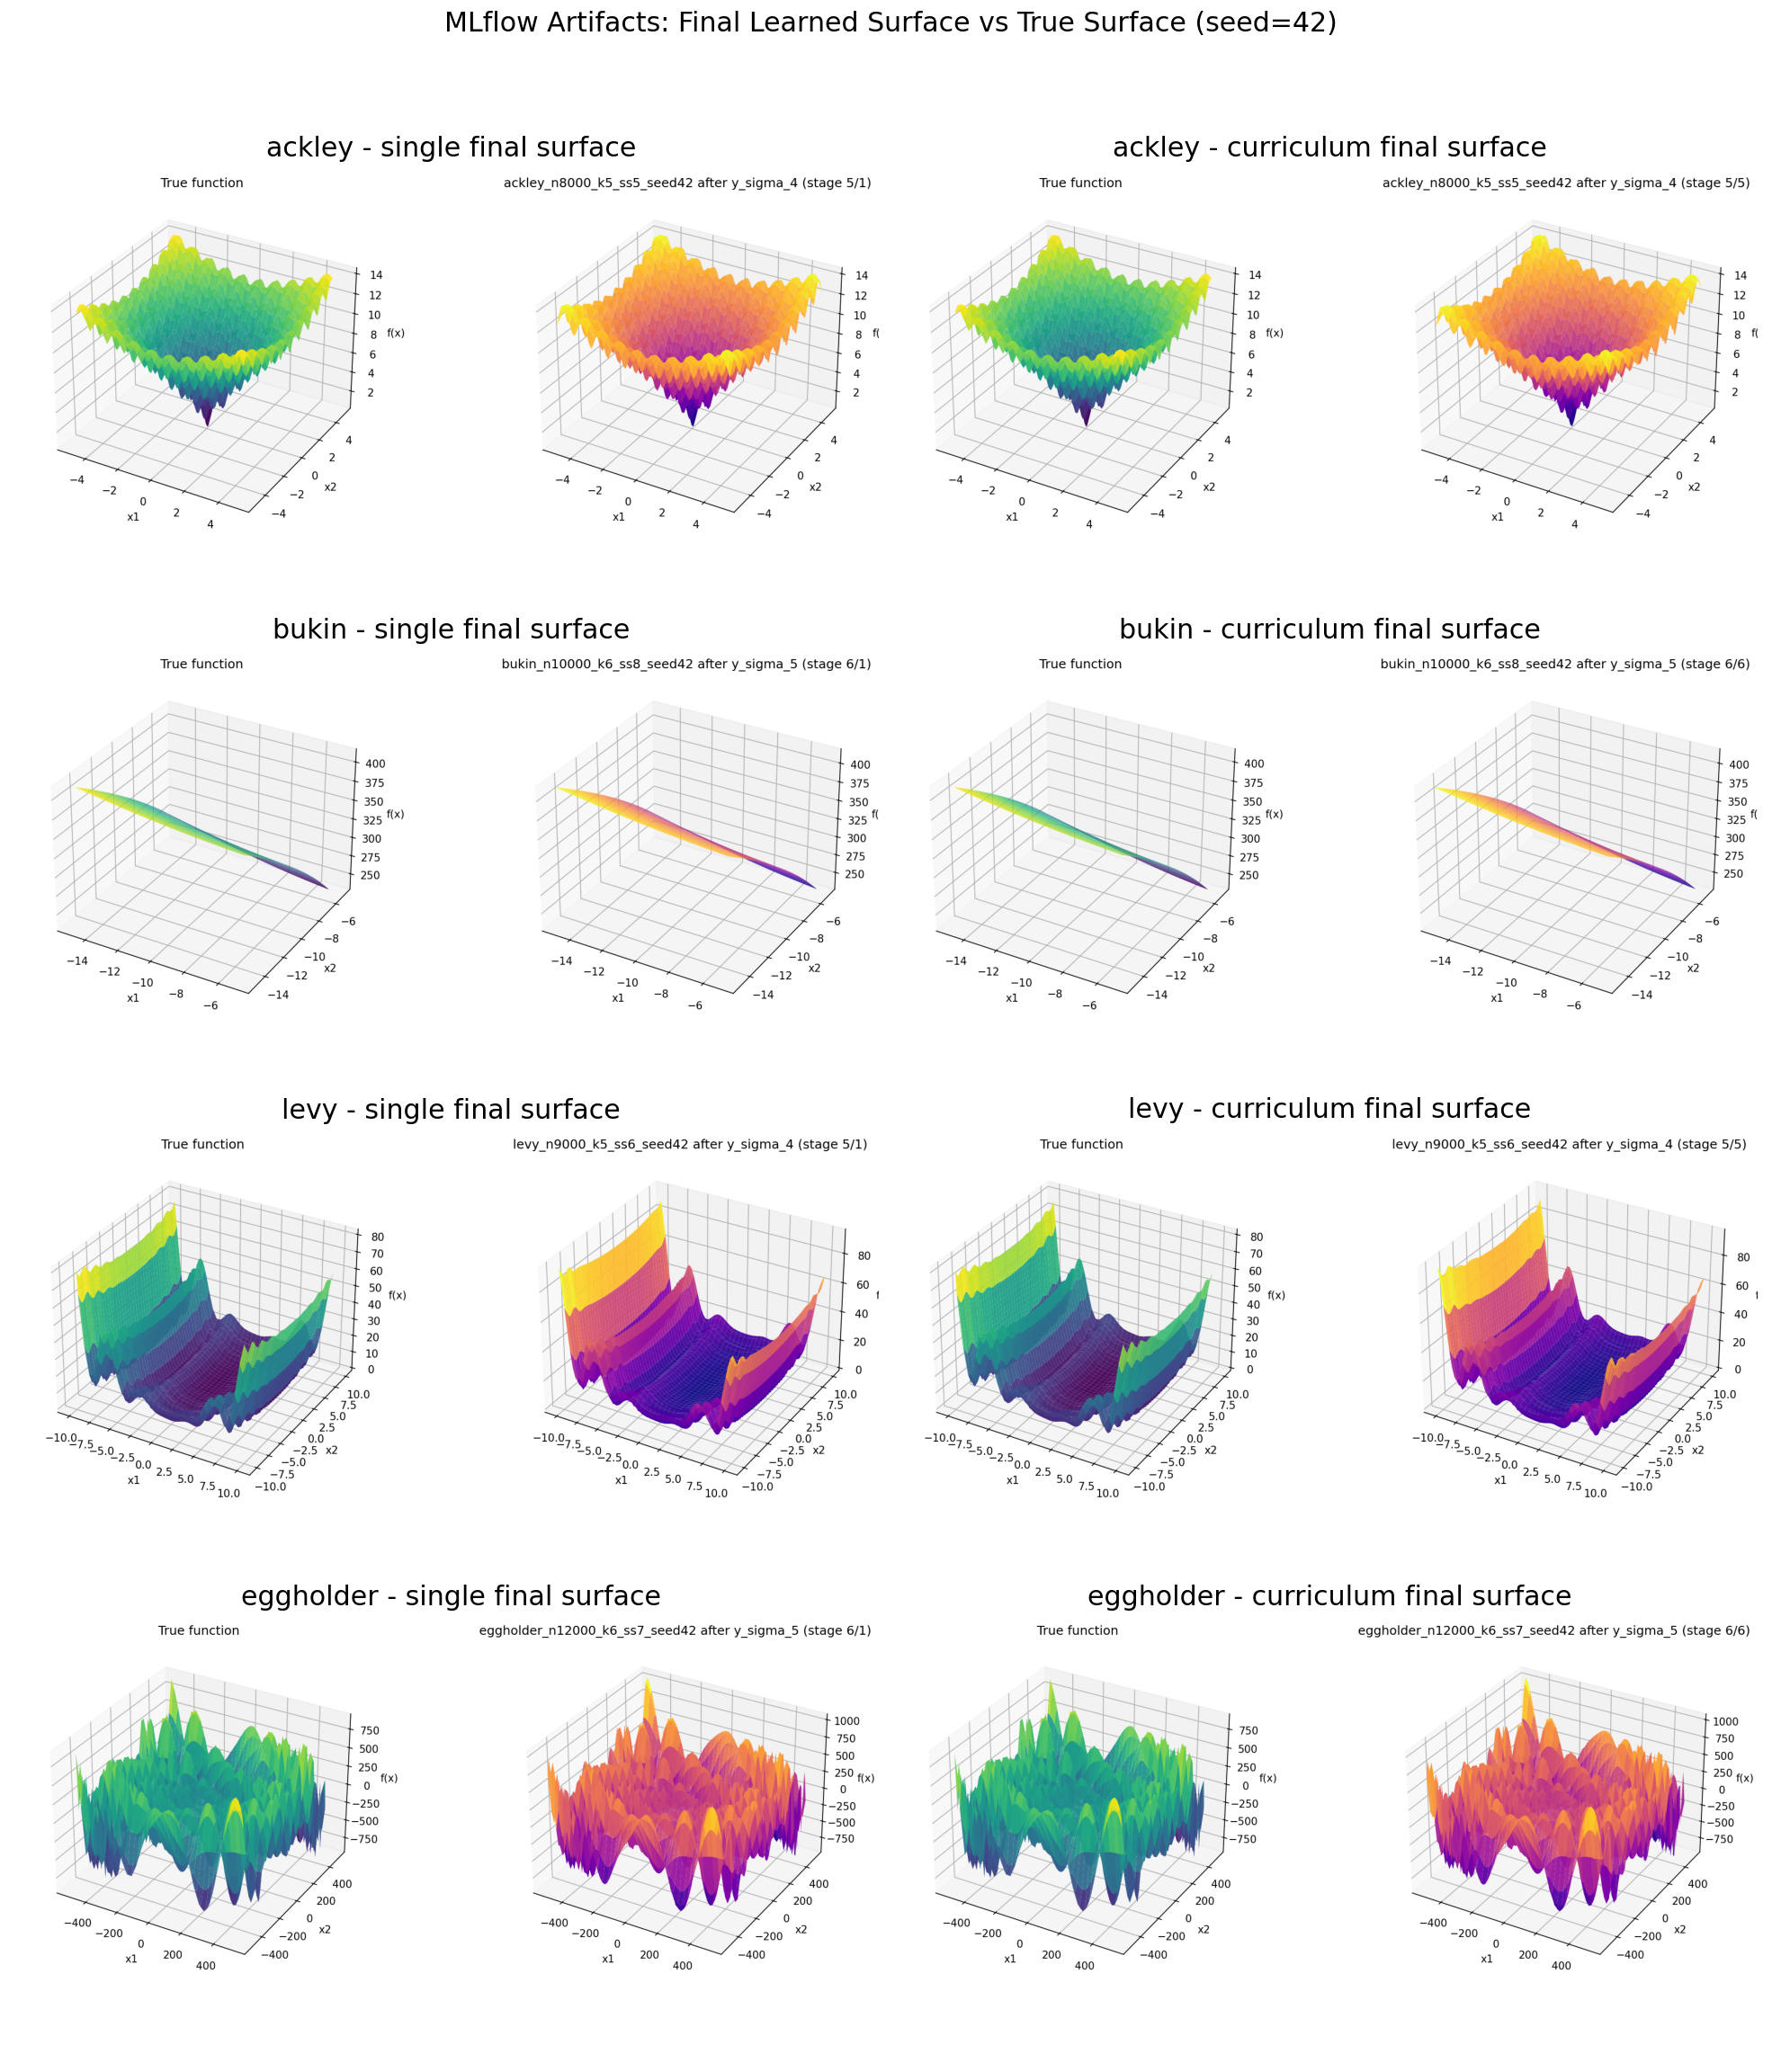
\includegraphics[width=0.98\textwidth]{figures/mlflow_curr_vs_single_final_surfaces_seed42.png}
    \caption{Final learned surfaces from MLflow artifacts. Each panel includes the learned surface and reference true surface used in training diagnostics.}
    \label{fig:mlflow-final-surfaces}
\end{figure}

\begin{figure}[h]
    \centering
    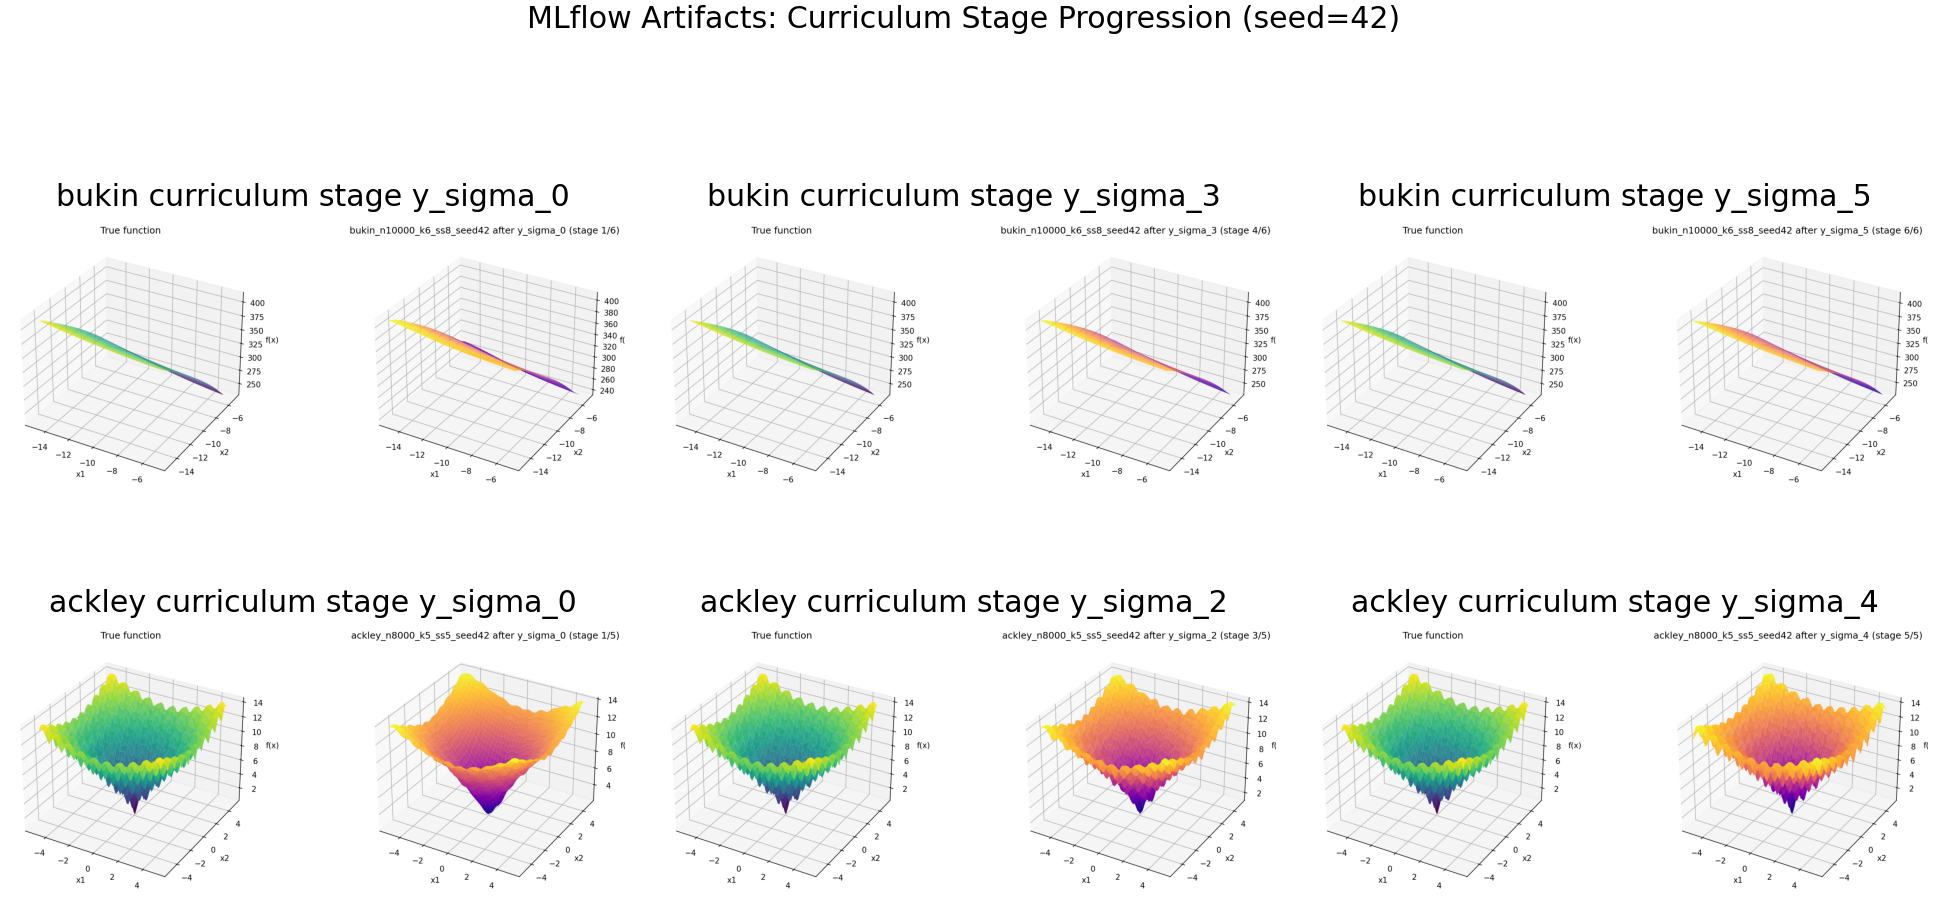
\includegraphics[width=0.98\textwidth]{figures/mlflow_curriculum_stage_progression_seed42.png}
    \caption{Curriculum stage progression for two representative functions (early, middle, final sigma stages).}
    \label{fig:mlflow-curriculum-stage}
\end{figure}

\begin{figure}[h]
    \centering
    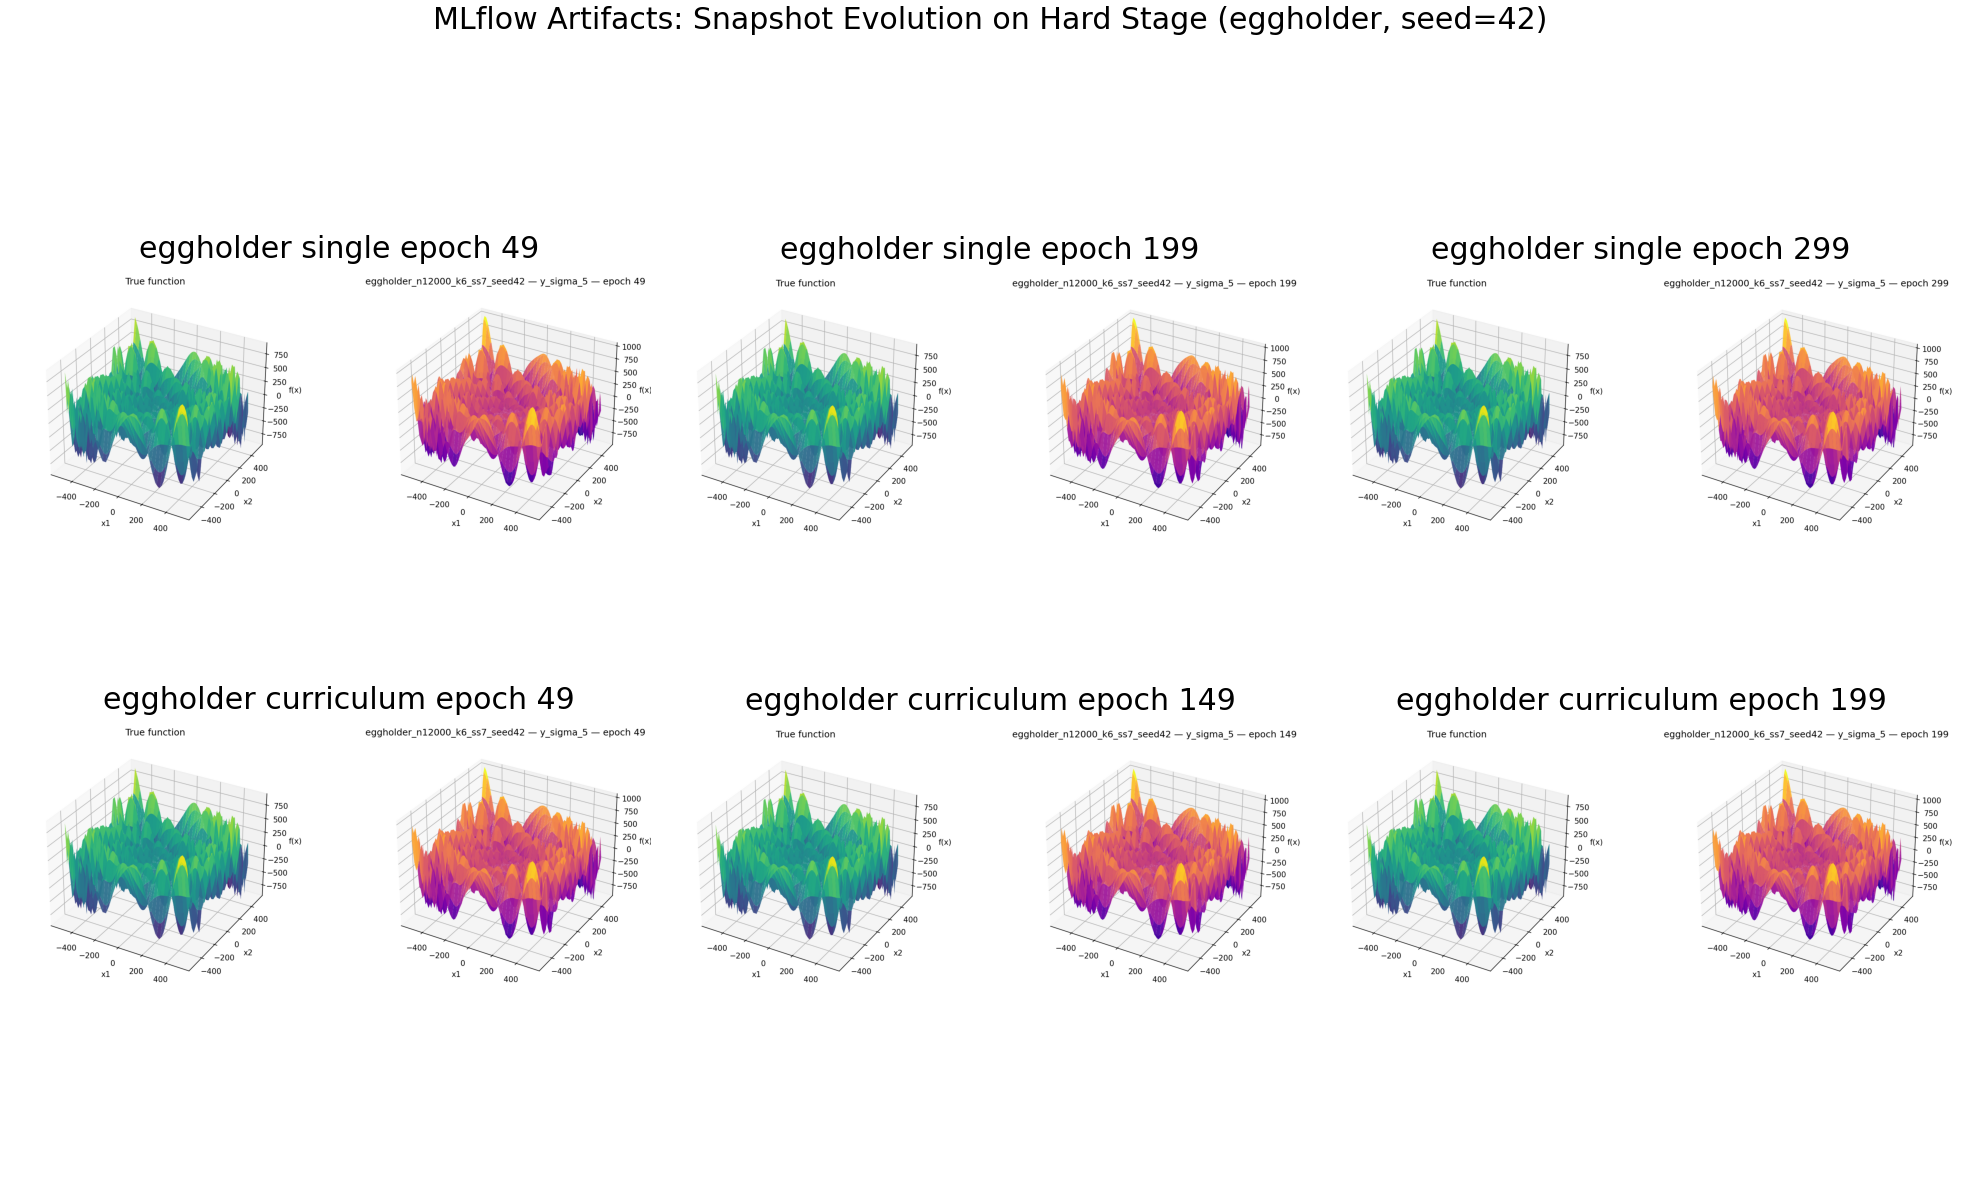
\includegraphics[width=0.98\textwidth]{figures/mlflow_eggholder_snapshot_evolution_seed42.png}
    \caption{Snapshot evolution on the hard stage for \texttt{eggholder} (single vs curriculum).}
    \label{fig:mlflow-eggholder-snapshots}
\end{figure}

\paragraph{What these artifact plots show.}
\begin{itemize}
    \item Curriculum often reaches smoother intermediate surfaces, but this comes
          with substantial extra compute time per run.
    \item For functions such as \texttt{bukin} and \texttt{levy}, curriculum trajectories
          can end closer to the target surface than single training.
    \item For \texttt{ackley} and \texttt{eggholder}, additional curriculum stages do
          not consistently translate into better hard-target final quality.
\end{itemize}

\section{Interpretation}

\paragraph{What worked.}
Curriculum provided repeatable quality gains for selected functions
(especially \texttt{bukin}, \texttt{franke}, and \texttt{levy}), indicating that
progressive smoothing can help optimization in some landscapes.

\paragraph{What did not work.}
Runtime increased in every function/regime cell.
In this benchmark, curriculum never won on runtime.

\paragraph{What this means.}
Curriculum should not be treated as a universal default. The current evidence
supports a selective policy:

\begin{itemize}
    \item use curriculum where quality gains are consistent,
    \item keep single-target training as the default baseline elsewhere,
    \item optimize curriculum schedule depth only where it materially helps.
\end{itemize}

\section{Limitations and next actions}

\begin{itemize}
    \item The \texttt{equal\_time} regime used a relatively high timeout cap,
          so it often did not enforce a tight budget.
    \item A stricter per-function cap (near single median runtime) should be used
          in the next iteration for stronger efficiency conclusions.
    \item The next cycle should test reduced-stage curriculum variants to lower runtime
          overhead while preserving gains on functions where curriculum helps.
\end{itemize}

\section{Strategic conclusion after two experiments}

After completing both stages reported in this thesis appendix
(the sweep-pack baseline and the curriculum-vs-single benchmark),
I conclude that the current baseline model capacity is too high to serve as a
useful foundation for curriculum-learning analysis. In practice, the baseline
single-target model often converges too strongly, leaving limited room for
curriculum to demonstrate consistent gains.

Therefore, the next research phase should focus on re-establishing a better
operating point before further curriculum claims are made.

\paragraph{Planned next phase.}
\begin{enumerate}
    \item \textbf{Capacity--data study:} determine an appropriate relation between
          dataset size and model parameter count for each function family.
    \item \textbf{Controlled re-sweep:} rerun hyperparameter sweeps under reduced
          model capacities and validated dataset sizes.
    \item \textbf{Training-loop refactor:} use this rerun to simplify and harden the
          experiment loop for cleaner reproducibility and easier ablation control.
    \item \textbf{Richer MLflow instrumentation:} log more detailed optimization
          diagnostics beyond losses, including roughness-related proxies
          (e.g., gradient variance, gradient-norm statistics, curvature/Hessian
          approximations, and stage-to-stage stability indicators).
    \item \textbf{Literature grounding first:} before implementation, conduct a short
          focused review on (a) parameter-count selection for regression settings
          and (b) quantitative loss-landscape roughness metrics.
\end{enumerate}

This plan is intended to produce a more informative baseline where curriculum
effects, if present, can be measured more reliably and interpreted with higher
confidence.
